\documentclass[laporan.tex]{subfiles}

\begin{document}

\chapter{Tinjauan Pustaka}

\section{Penelitian Terkait}

\subsection{Improving quality inspection of food products by computer vision – a review}

Kualitas produk pangan diukur dari penampilan, bau, tekstur, rasa dan berbagai aspek subjektif lainnya yang dinilai oleh manusia. Namun inspeksi dengan tenaga manusia mempunyai banyak kelemahan antara lain ongkos yang tinggi serta  hasil yang tidak konsisten.

Makalah ini\cite{brosnan} membahas berbagai penelitian di bidang computer vision yang diterapkan untuk menggantikan inspeksi manual pada berbagai produk pangan dan pertanian.

Beberapa penelitian memfokuskan pada deteksi cacat bentuk atau tekstur secara visual. Ekspansi Fourier dapat mendeteksi bentuk kultivar apel dengan kesuksesan 90\%.

\subsection{Identifikasi Iris Mata Menggunakan Alihragam Wavelet Haar}

Penelitian ini mencoba pemanfaatan transformasi wavelet Haar untuk pengenalan iris. Pada penelitian ini ciri energi hasil transformasi wavelet menjadi masukan dari perhitungan jarak Euclidean. Akurasi berbagai jenis format citra dan tingkatan dekomposisi diuji dengan hasil menunjukkan bahwa format citra tanpa kompresi dan dekomposisi tingkat 4 menghasilkan hasil yang paling akurat yaitu 85.58\%.\cite{prihartono}

\subsection{Navel Orange Blemish Identification for Quality Grading System}

Menurut penelitian ini, klasifikasi pixel untuk mengenali memar pada kulit jeruk mempunyai akurasi rendah karena perbedaan intensitas warna antara bagian tengah jeruk dengan bagian tepi jeruk pada citra jeruk. Untuk mengatasi masalah tersebut pengetahuan a priori mengenai variasi intensitas pada benda bulat diterapkan agar pixel bagian yang cacat dapat dikenali dengan tepat. Metode yang digunakan berhasil mengenali 96\% dari jeruk yang baik dan 97\% dari jeruk dengan cacat.

\subsection{A Wavelet Approach to Edge Detection}

Tesis ini menjelaskan mekanisme deteksi tepi dari sudut pandang transformasi wavelet dan metode deteksi tepi multi-level berbasis wavelet. Menurut tesis ini, \emph{dyadic scale} yang digunakan pada transformasi wavelet tidak selalu dapat diadaptasikan secara optimal untuk citra dengan banyak \emph{noise}. Tesis ini mengusulkan penggunaan algoritma \emph{cascade} yang dapat menemukan skala yang tepat untuk sinyal dan tingkat \emph{noise} tertentu.

\subsection{Edge detection by scale multiplication in wavelet domain}

Penelitian ini mengajukan metode deteksi tepi citra dengan perkalian dua hasil transformasi wavelet pada skala berdekatan untuk memperjelas struktur tepi dan meredam \emph{noise} (derau). Tepi dan noise memiliki karakteristik transformasi wavelet yang beda, dengan struktur tepi muncul pada setiap skala sementara \emph{noise} lenyap pada skala yang lebih besar. Metode yang disarankan mengambil maksimum lokal hasil perkalian dua \emph{subband} DWT setelah melalui proses \emph{thresholding}.

\section{Computer Vision}

Citra digital adalah fungsi intensitas warna dua dimensi f(x,y) dimana x dan y mewakili koordinat lokasi suatu titik dan nilai dari fungsi yang merupakan tingkat intensitas warna atau tingkat keabu-abuan dari titik tersebut (Schalkoff, 1989). Citra digital merupakan representasi dari suatu objek nyata yang dapat dikenali oleh komputer.

Pengolahan citra digital atau digital image processing pengolahan sinyal untuk input citra digital dua dimensi. Tujuan pengolahan citra digital adalah untuk meningkatkan kualitas gambar sehingga lebih mudah dilihat oleh manusia atau lebih mudah diolah oleh komputer.

Computer vision adalah bidang studi yang mempelajari metode-metode pengumpulan, pemrosesan, analisis dan penafsiran citra dari dunia nyata dengan tujuan untuk menghasilkan informasi numerik atau simbolis.

Berikut ini adalah pengertian computer vision menurut beberapa pakar

\begin{enumerate}
\item Ballard dan Brown, computer vision adalah otomatis dan integrasi sebuah range yang luas yang terdiri dari proses-proses dan representasi-representasi terhadap persepsi visual.
\item Adrian Low, computer vision berhubungan dengan perolehan gambar, pemrosesan, klasifikasi, pengenalan, dan menjadi penggabungan, pengurutan, pembuatan keputusan menuju pengenalan.
\item Shapiro dan Stockman, computer vision adalah suatu bidang yang bertujuan untuk membuat suatu keputusan yang berguna mengenai objek fisik nyata dan keadaan berdasarkan atas sebuah citra. Computer vision merupakan kombinasi antara pengolahan citra dan pengenalan pola. Hasil keluaran dari proses computer vision adalah pengertian tentang citra.
\end{enumerate}

Boyle dan Thomas mengatakan bahwa computer vision lebih daripada pengenalan, computer vision melakukan operasi “low level processing” sebagai algoritma image processing yang murni. Mereka juga yang menggolongkan image processing ke dalam computer vision.

\section{Tepi dan Pendeteksian Tepi}

Tepi (\emph{edge}) adalah kontur pada citra tempat terjadinya perubahan kecerahan citra secara drastis. Dalam pengolahan citra, tepi sering diinterpretasikan sebagai suatu singularitas. Singularitas sebuah fungsi dapat dikarakterisasi sebagai diskontinuitas dengan gradien yang mendekati tak hingga. Pada data citra yang bersifat diskrit, tepi didefinisikan sebagai maksima lokal sebuah gradien.

Pendeteksian tepi merupakan perkakas penting dalam pengenalan pola. Pendeteksi tepi pada dasarnya adalah \emph{high-pass filter} yang dapat digunakan untuk mengambil titik-titik tepi pada citra. Pada penelitian ini akan digunakan \emph{wavelet} untuk melakukan pendeteksian tepi.

\section{Transformasi Wavelet}

Wavelet merupakan sekumpulan fungsi dalam ruang $L^2(R)$ yang memiliki sifat-sifat berikut:

\begin{enumerate}
\item Berenergi terbatas
\item Merupakan fungsi band-pass
\item Merupakan hasil translasi dari sebuah fungsi tunggal
\end{enumerate}

Wavelet digunakan untuk membagi sebuah fungsi atau sinyal menjadi komponen-komponen frekuensi yang berbeda dan mempelajari tiap komponen dengan resolusi yang sesuai skala masing-masing.

Transformasi wavelet merupakan salah satu teknik untuk merepresentasikan sinyal ke dalam domain frekuensi dan waktu. Proses transformasi wavelet melewatkan sinyal pada filter dengan skala frekuensi yang berbeda, kemudian ditransformasikan dengan fungsi wavelet yang ukurannya disesuaikan dengan rentang frekuensi komponen sinyal.

Transformasi wavelet mengatasi kelemahan pada transformasi Fourier yang tidak memiliki resolusi waktu, serta transformasi Fourier waktu singkat yang resolusi frekuensinya hanya baik pada rentang frekuensi tertentu. Transformasi wavelet adalah solusi yang cocok untuk sinyal non-stasioner.

Transformasi wavelet kontinu didefinisikan sebagai berikut
% equation
\begin{equation}
\gamma(s, \tau) = \int f(t) \phi^{*}_{s,\tau}(t)dt
\end{equation}

Invers dari TWK didefinisikan sebagai berikut
% equation
\begin{equation}
f(t) = \int \int \gamma(s,\tau)\phi_{s,\tau}(t)d {\tau}ds
\end{equation}

Fungsi dasar wavelet dapat didefinisikan sesuai kebutuhan. Secara matematika fungsi wavelet didefinisikan sebagai berikut
%equation
\begin{equation}
\phi_{s,\tau}(t) = \frac{1}{s}\phi(\frac{t-\tau}{s})
\end{equation}

Transformasi wavelet diskrit adalah transformasi wavelet pada sinyal diskrit. Filterisasi wavelet direalisasikan dengan pasangan Quadrature Mirror Filter (QMF) yaitu pasangan filter yang memenuhi persamaan berikut
%equation
\begin{equation}
h[L-1-n]=(-1)^ng[n]
\end{equation}

Pembagian sinyal menjadi frekuensi tinggi dan rendah ini disebut sebagai dekomposisi. Proses dekomposisi dimulai dengan melewatkan sinyal melewati HPF dan LPF. Sinyal keluaran dari masing-masing filter memiliki rentang frekuensi setengah dari sinyal asli. Setelah filterisasi, setengah dari sample atau subsample dapat dieliminasi berdasarkan aturan Nyquist. Dengan demikian sinyal selalu dapat di-subsample dengan factor 2 dengan cara mengabaikan setengah sample lainnya. Proses dekomposisi ini dapat dilakukan sebanyak satu tingkatan atau lebih. Secara matematika prosesnya adalah
%equation
\begin{equation}
y_{tinggi}[k]=\sum_n x[n]h[2k-n]
y_{rendah}[k]=\sum_n x[n]g[2k-n]
\end{equation}

Contoh dekomposisi wavelet tingkat tiga
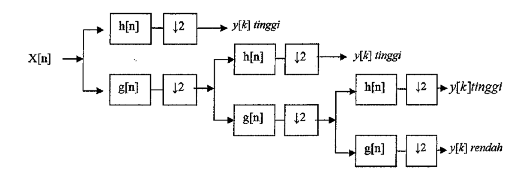
\includegraphics[width=8cm]{tex/decomp2d.png}

$y[k]$ adalah hasil dekomposisi. $y[k]$ tinggi adalah detil dari informasi sinyal sedangkan $y[k]$ rendah merupakan taksiran kasar dari fungsi penskalaan. Dengan menggunakan koefisien TWD ini dapat dilakukan proses invers untuk merekonstruksi sinyal asal. Persamaan rekonstruksi pada masing-masing tingkatan dapat ditulis sebagai berikut

\begin{equation}
x[n]=\sum_k (y_{tinggi}[k]h[-n+2k]+y_{rendah}[k]g[-n+2k])
\end{equation}

Dekomposisi pada citra menghasilkan informasi rentang frekuensi yang berbeda yaitu frekuensi rendah-rendah (LL), frekuensi rendah-tinggi (LH), frekuensi tinggi-rendah (HL), dan frekuensi tinggi-tinggi (HH). Rentang LL merupakan rentang taksiran penskalaan sedangkan rentang LH, HL dan HH merupakan rentang frekuensi detil informasi.

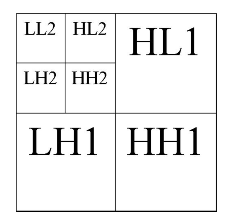
\includegraphics[width=8cm]{tex/ll.png}

Transformasi wavelet diskrit sering dipilih karena beberapa alasan

\begin{enumerate}
\item TWD paling dekat dengan \emph{human visual system}
\item Distorsi yang disebabkan oleh domain wavelet dalam perbandingan kompresi tinggi tidak terlalu mengganggu dibandingkan domain lain pada bit rate yang sama.
\item Bit-error rate yang rendah. Bit-error rate merupakan perbandingan antara bit yang salah diekstraksi dengan total bit yang disisipkan.
\end{enumerate}

\section{Deteksi Tepi}


\section{Transformasi Wavelet untuk Deteksi Tepi}

\subsection{Perancangan Wavelet}

Cardinal B-splines dengan orde m, $N_m(x)$, didefinisikan secara induktif melalui konvolusi fungsi kotak:

\begin{equation}
	N_1(x)=B(x)=\begin{cases}
		1, 0 \leq x \leq 1 \\
		0, untuk selainnya
	\end{cases} ,
	N_m(x)=N_{m-1} \ast N_1(x)
\end{equation}

Cardinal B-splines semakin mendekati fungsi Gaussian $\phi_n(x)$ untuk $n$ mendekati tak hingga.

Gaussian wavelet untuk skala integer $n > 2$ dapat diperoleh dengan pendekatan

\begin{align}
	\psi_n(x) & \approx \overbrace{N_1 \ast \ldots  N_1}^{n-2} \ast H(x) \\
	& = N_{n-2} \ast H(x)
\end{align}

dengan $H(x)$ merupakan wavelet Haar

\begin{align}
	H(x) & = \begin{cases}
		-1, 0 \leq x \leq \frac{1}{2}; \\
		1, \frac{1}{2} \leq x \leq 1; \\
		0, selainnya
	\end{cases} \\
	\psi_1(x) & \approx H(x)
\end{align}

$\psi(x)$ merupakan wavelet Gaussian dengan skala 1.

Selanjutnya persamaan di atas dapat dikembangkan untuk fungsi 2D sebagai berikut:

\begin{align}
	N_1(x,y) & = B(x,y) = \begin{cases}
		1, 0 \leq x \leq 1, 0 \leq y \leq 1; \\
		0, selainnya \\
	\end{cases} \\
	H^1(x,y) & = \begin{cases}
		-1, 0 \leq x \leq \frac{1}{2}, 0 \leq y \leq 1;
		1, \frac{1}{2} \leq x \leq 1, 0 \leq y \leq 1;
		0, selainnya \\
	\end{cases} \\
	H^2(x,y) & = \begin{cases}
		-1, 0 \leq x \leq 1, 0 \leq y \leq \frac{1}{2};
		1, 0 \leq x \leq 1, 0 \leq y \leq \frac{1}{2};
		0, selainnya \\
	\end{cases} \\
\end{align}

Dengan demikian,

\begin{align}
	W^1f(n,x,y) & \approx \overbrace{N_1 \ast \ldots \ast N_1}^{n-2} \ast H^1 \ast f(x,y);
	W^2f(n,x,y) & \approx \overbrace{N_1 \ast \ldots \ast N_1}^{n-2} \ast H^2 \ast f(x,y);
\end{align}

Kedua persamaan di atas digunakan untuk mengukur transformasi wavelet horizontal dan vertikal pada skala $n$.

\subsection{Algoritma Deteksi Tepi dengan Wavelet}

\subsection{Algoritma Deteksi Tepi Canny}

Algoritma deteksi tepi Canny terdiri dari lima langkah, yaitu

\begin{description}
\item [Penghalusan:] menghaluskan citra untuk menghilangkan \emph{noise}.
\item [Perhitungan gradien:] perhitungan gradien perubahan nilai intensitas pada tiap titik.
\item [Supresi non-maksimum:] penghilangan hasil perhitungan gradien yang bukan merupakan maksium lokal.
\item [\emph{Double thresholding:}] penentuan tepi berdasarkan ambang batas.
\item [Pelacakan tepi berdasarkan histeresis:] menghilangkan tepi lemah yang tidak terhubung dengan tepi yang kuat.
\end{description}

Penghalusan dilakukan dengan menggunakan filter \emph{Gaussian}. Penghalusan bertujuan untuk menghilangkan \emph{noise} agar tidak mempengaruhi hasil deteksi tepi.

Perhitungan gradien dilakukan pada citra yang telah dihaluskan dengan operator Sobel. Citra difilter dengan dua \emph{mask} yang mengukur gradien pada arah sumbu $x$ dan sumbu $y$.

\begin{equation}
\begin{split}
K_{GX} = \begin{bmatrix}
-1 & 0 & 1 \\
-2 & 0 & 2 \\
-1 & 0 & 1
\end{bmatrix}
\\
K_{GY} = \begin{bmatrix}
1 & 2 & 1 \\
0 & 0 & 0 \\
-1 & -2 & -1
\end{bmatrix}
\end{split}
\end{equation}

Operator Sobel menghasilkan nilai gradien pada arah $x$ dan $y$, namun besar gradien ini belum merupakan garis tipis yang menunjukkan tepi. Tepi yang sebenarnya dapat dicari dari nilai maksimum lokal gradien pada arah yang sama. Arah gradien didapatkan dari pengukuran nilai $arctan$ gradien pada kedua arah yang selanjutnya dibulatkan menjadi delapan arah diskrit dengan sudut sebesar 45$^o$. Nilai yang bukan maksimum lokal dibuang dari citra gradien.

\emph{Double thresholding} dilakukan untuk membuang nilai-nilai yang tidak diinginkan, misalnya tepi yang timbul dari perbedaan intensitas cahaya. Pemilihan nilai ambang batas sangat menentukan akurasi identifikasi tepi-tepi yang relevan dari objek.

\section{Identifikasi Daerah Cacat Pada Kulit Jeruk}

Setelah batas-batas warna kulit jeruk didapatkan melalui deteksi tepi, langkah selanjutnya adalah menentukan apakah region yang dibatasi oleh tepi merupakan kulit yang normal atau cacat. Untuk itu dilakukan dua langkah yaitu penentuan region cacat berdasarkan nilai intensitas pixel dari tiap region warna dan penandaan seluruh pixel yang ada pada region tersebut.

\subsection{Identifikasi Daerah Cacat Berdasarkan Nilai Pixel}

\subsection{Operasi \emph{Hole Filling} untuk Menandai Daerah Cacat}

Daerah cacat yang telah dibatasi oleh tepi dapat diangggap sebagai sebuah lubang. Dari sebuah titik tepi $(x, y)$ titik $(x+1, y)$ ditandai sebagai titik cacat atau normal, lalu seluruh daerah yang dibatasi tepi tersebut ditandai seperti titik $(x+1, y)$.

\begin{equation}
X_k = (X_{k-1} \oplus B) \cap A^c  k=1,2,3,\ldots
\end{equation}

\subsection{Pengukuran Luas Daerah Cacat}
% operasi spasial untuk mask
% klasifikasi mask berdasarkan jenis pixel

\end{document}
